% % % % % % % % % % % % % % % % % %
%                                 %
%  Master Thesis                  %
%  MSc in Aerospace Engineering   %
%  Mattia Gregnanin               %
%  A.Y. 2025/2026                 %
%                                 %
% % % % % % % % % % % % % % % % % %
%                                 %
%  Chapter 1                      %
%                                 %
% % % % % % % % % % % % % % % % % %

\graphicspath{{chapters/1/figures/}}

\chapter[State of the Art and Design Motivations]{State of the Art in Rocket Flight Computers and Design Motivations}
\label{ch:state-of-the-art}

This thesis presents the design of a flight computer for an amateur rocket developed by a small team of students. Its objective is to acquire measurements from onboard sensors, to reconstruct the attitude, position and velocity of the rocket in real time, and to transmit them to a ground station by radio. This chapter places this work in the context of existing solutions and motivates the design choices that were made.

Flight computers for amateur rocketry are rarely documented in the scientific literature. The review therefore relies mainly on manufacturers' manuals and datasheets, on the repositories and documentation published by open-source projects and student teams, and on the technical literature on inertial navigation and sensor fusion. 

The chapter is organised as follows. \cref{sec:history} outlines the historical development of flight computers, from the guidance systems of the first rockets to the devices available to amateur rocketry. \cref{sec:components} describes the functional blocks that compose a flight computer. \cref{sec:existing} reviews commercial products and open-source or student projects, and compares them in terms of sensors, estimation capabilities and telemetry. Finally, \cref{sec:choices} defines the requirements of the flight computer developed in this work and motivates the choice of the microcontroller, of the sensors and of the radio module. The design of the power supply, of the recovery electronics and of the data storage is described in \cref{ch:hardware}, while the estimation algorithms and the firmware are presented in \cref{ch:estimation,ch:firmware}.

% % % % % % % % % % % % % % % % % %
%                                 %
%  Master Thesis                  %
%  MSc in Aerospace Engineering   %
%  Mattia Gregnanin               %
%  A.Y. 2025/2026                 %
%                                 %
% % % % % % % % % % % % % % % % % %
%                                 %
%  Chapter 1 / Section 1          %
%                                 %
% % % % % % % % % % % % % % % % % %

\section{Historical Overview}
\label{sec:history}

The history of rocket flight computer systems is closely tied to the development of rocketry and the advancement of electronic technology. One of the earliest examples of a rocket guidance system was the \emph{Mischgerät}, an electromechanical device used in the German V-2 rocket during World War II (\cref{fig:mischgerat}). It processed electrical signals from onboard spinning gyroscopes to control the rocket's flight path~\cite{cdvandt}. German engineers also pioneered radio telemetry on board rockets, transmitting sensor measurements from the vehicle to a ground station~\cite{rocketryhandbook}. Although these systems represented a significant technological achievement for their time, their complexity, weight, and specialized hardware made them unsuitable for widespread use outside military and research applications.

Following World War II, guidance and navigation systems continued to evolve alongside advances in electronics and computing. A notable milestone was the Apollo Guidance Computer (AGC), developed for NASA's Apollo missions during the 1960s. Shown in \cref{fig:agc}, it was among the first computers to make extensive use of integrated circuits, demonstrating how electronic computing could be integrated into spacecraft guidance and navigation systems~\cite{digitalapollo}. Nevertheless, the cost, complexity and specialized nature of these systems placed them well beyond the reach of amateur rocketry.

\begin{figure}[htb]
    \centering
    \begin{subfigure}{0.48\textwidth}
        \centering
        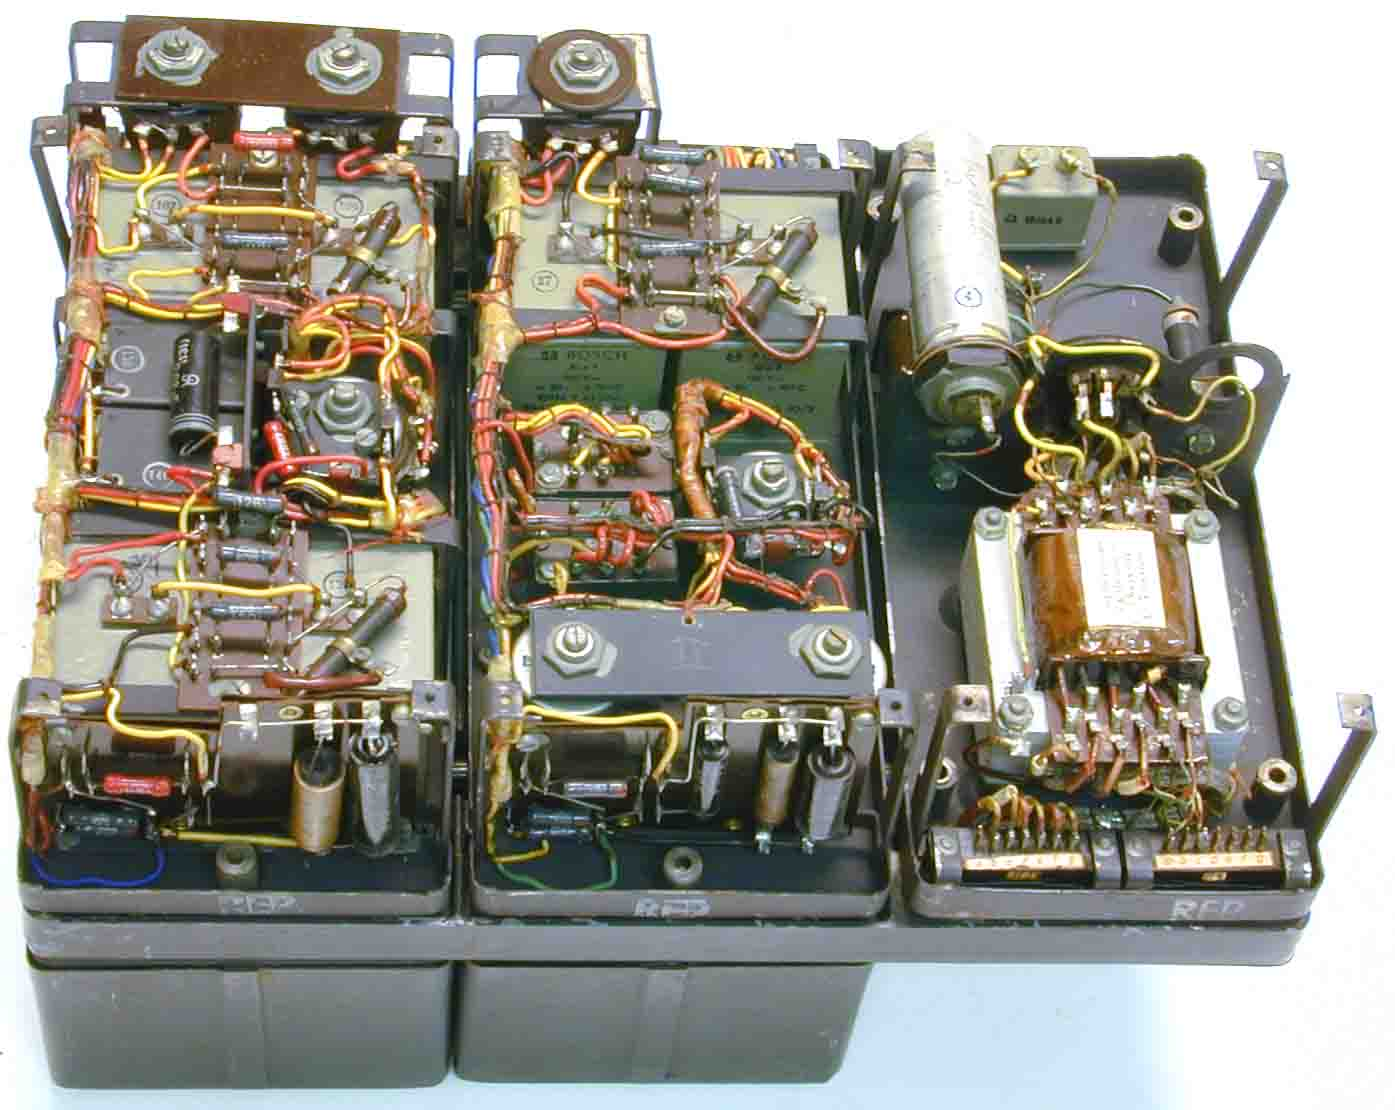
\includegraphics[width=\textwidth]{mischgerat}
        \caption{V-2 rocket control unit (Mischgerät)~\cite{cdvandt}.}
        \label{fig:mischgerat}
    \end{subfigure}
    \hfill
    \begin{subfigure}[b]{0.48\textwidth}
        \centering
        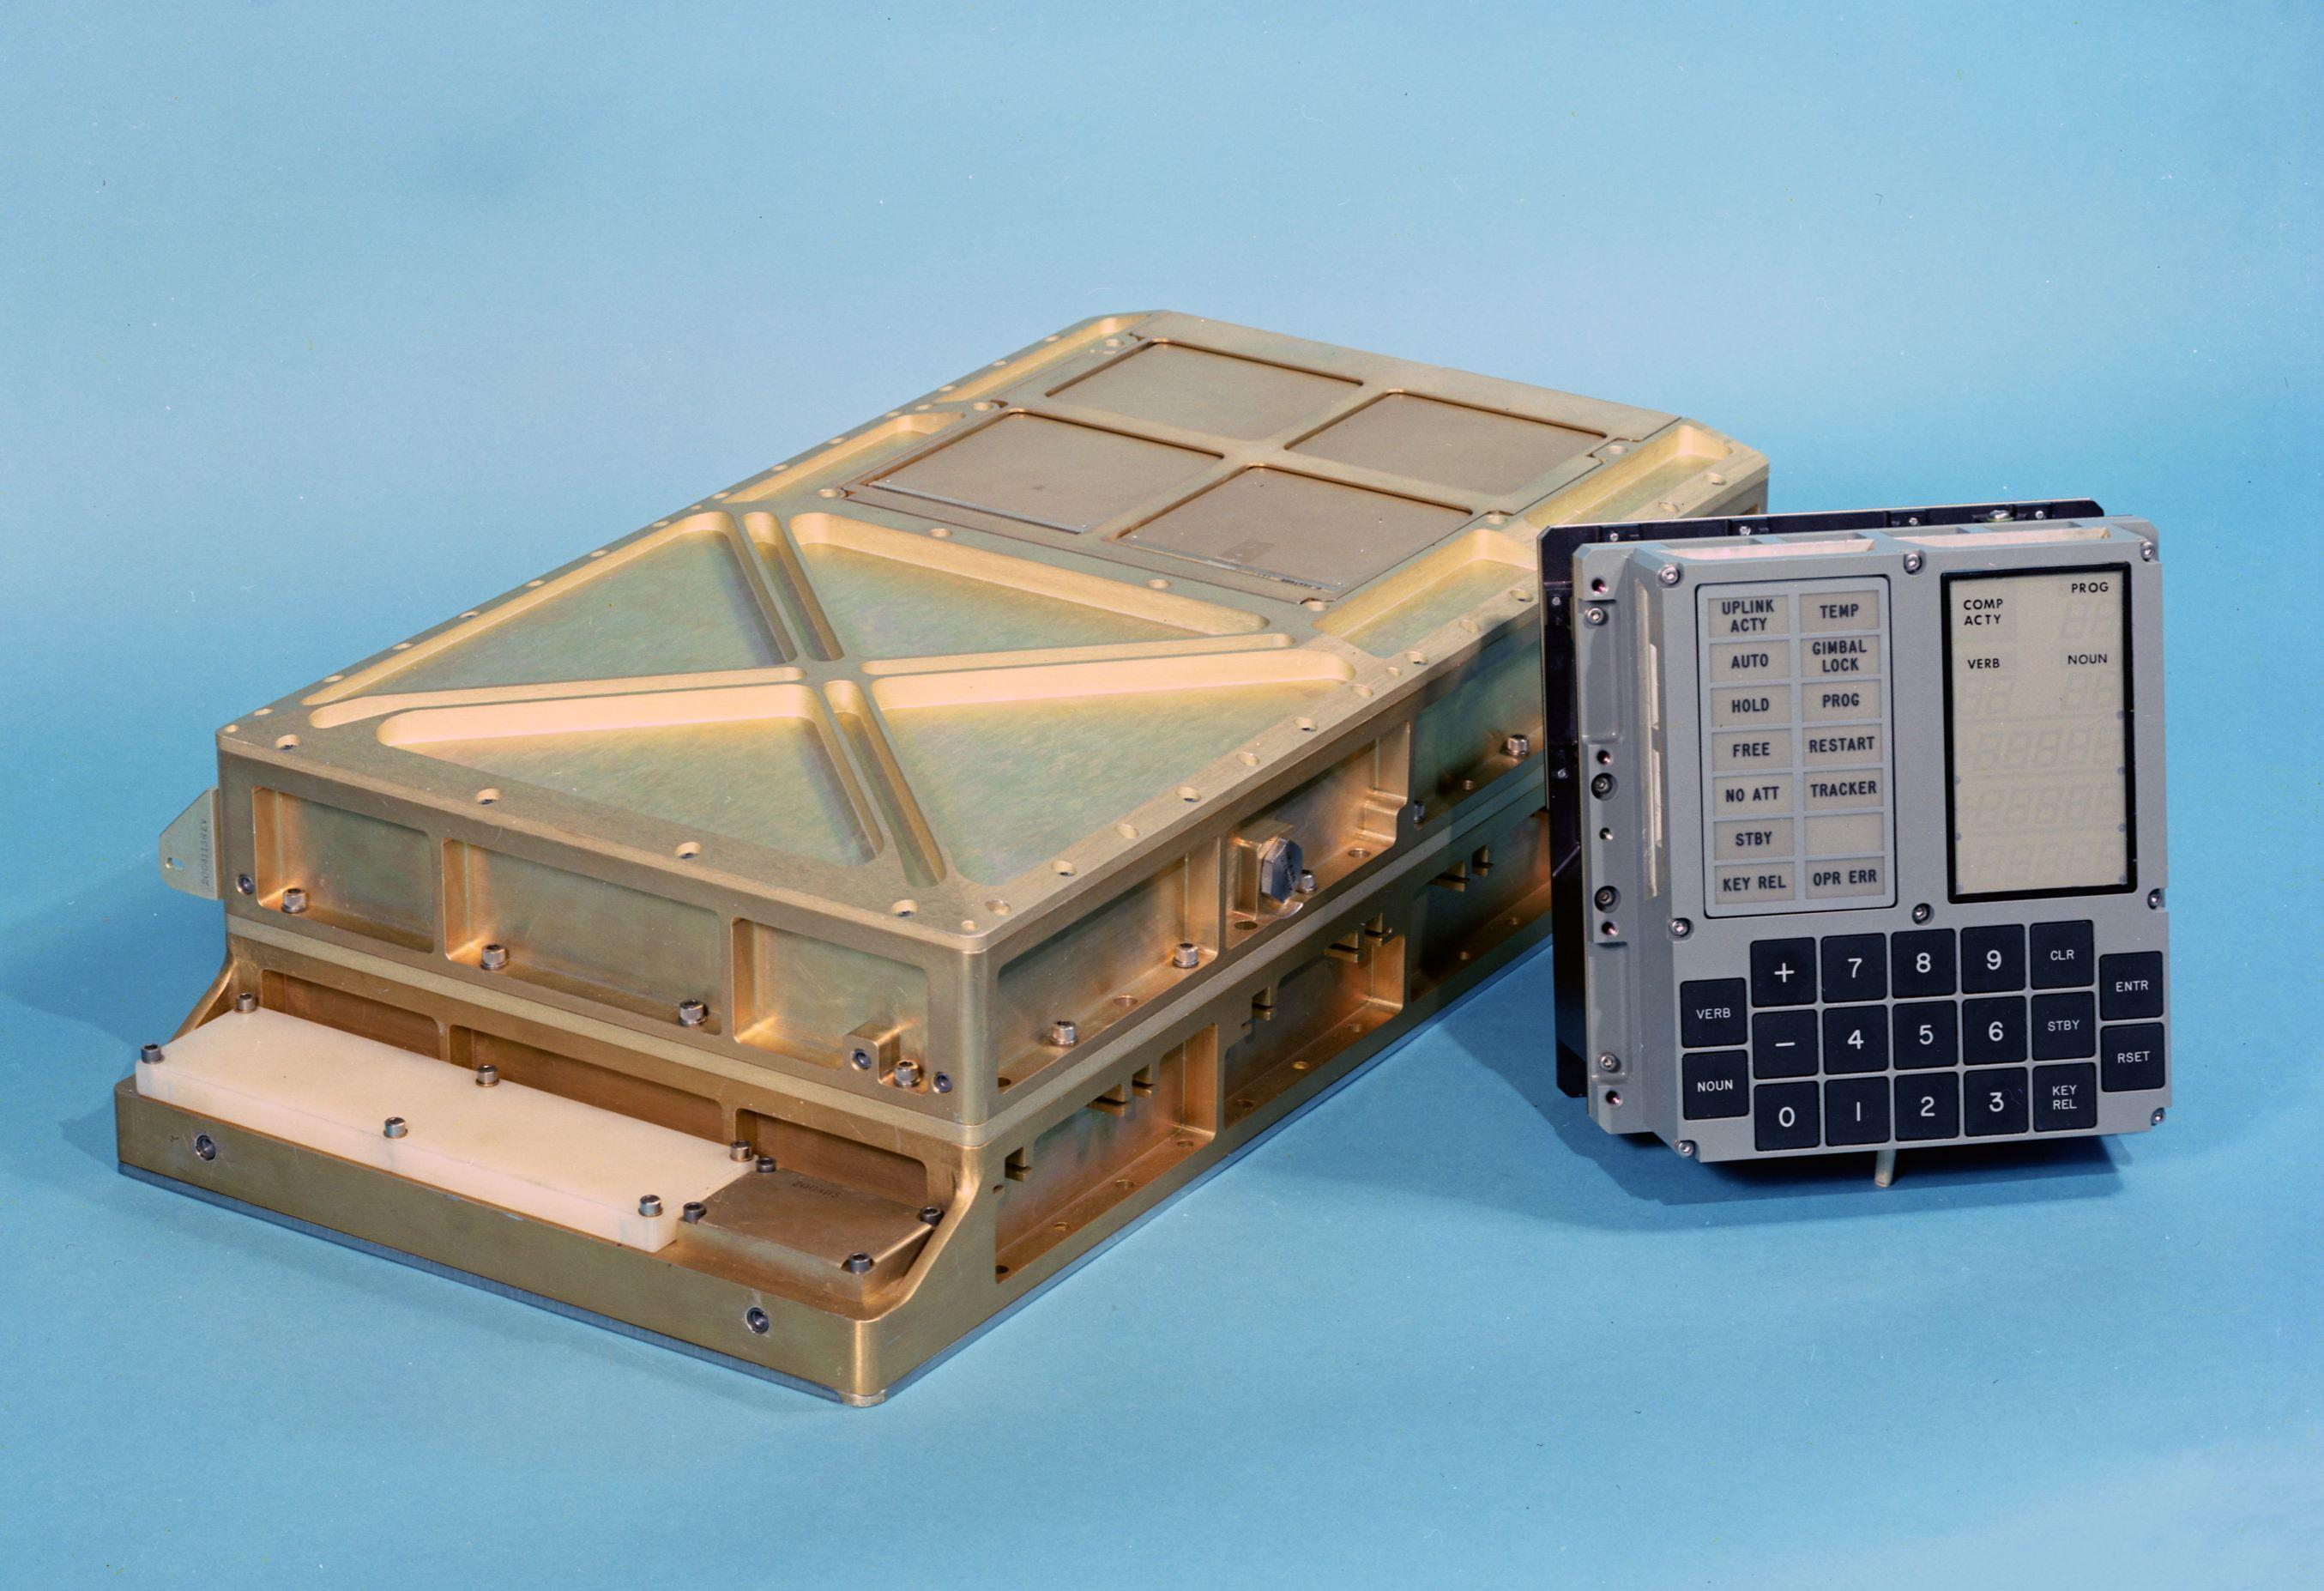
\includegraphics[width=\textwidth]{agc}
        \caption{Apollo Guidance Computer~\cite{wiki:agcview}.}
        \label{fig:agc}
    \end{subfigure}
    \caption{Historical examples of guidance systems for rockets and spacecraft.}
    \label{fig:historicalguidance}
\end{figure}

In parallel, electronics began to play an important role in amateur rocketry, initially as a means of recovering rockets after landing. The first amateur rocket transmitter, built in Colorado in 1960, emitted a signal in the \SI{27}{MHz} Citizen Band (CB) frequency band. The signal could be detected using a directional antenna to locate the rocket on the ground~\cite{rocketryhandbook}. Unlike modern telemetry systems, this initial device served only as a recovery beacon and did not transmit, at least in its early versions, flight measurements.

Beyond locating the rocket, a more fundamental requirement is its safe recovery. Model rocketry associations such as the NAR and Tripoli require that rockets be recovered in a safe manner after each flight, which also allows them to be flown again~\cite{nar:safetycode,tripoli:safetycode}.
Traditionally, recovery was triggered by the delay element built into the motor, which fires an ejection charge after burnout~\cite{rocketryhandbook}, or by simple mechanical or electronic timers. In both cases the deployment time is fixed before launch, whereas the instant of apogee depends on factors such as vehicle mass, aerodynamic drag, weather conditions and motor variability. Deployment can therefore occur too early or too late, compromising the integrity of the vehicle and the safety of the surroundings.

The subsequent development of microprocessors, microcontrollers and miniaturized sensors in the following decades progressively reduced the size, cost and power consumption of onboard electronic systems. In particular, the availability of compact inertial sensors and pressure sensors in the form of \emph{Micro Electro-Mechanical Systems} (MEMS) made it possible to integrate measurement, data processing and event detection into small, affordable devices~\cite{nato:mems}. These advances enabled amateur flight computers to measure altitude, record flight data and trigger recovery systems based on measured flight conditions rather than relying exclusively on predetermined delays.

More recently, open-source hardware and software have further lowered the barriers to developing custom flight computers. Development platforms such as Arduino and ESP32 provide accessible environments for prototyping embedded systems, while single-board computers such as Raspberry Pi can support more computationally demanding applications, including onboard video and image recording. Alongside custom-built solutions, several commercial products have been developed specifically for amateur rocketry, including the Altus Metrum TeleMetrum~\cite{altus:telemetrum}, the PerfectFlite StratoLoggerCF~\cite{perfectflite} and the Featherweight Blue Raven~\cite{featherweight:blueraven}, that will be reviewed in \cref{sec:existing}. Depending on the model, these devices combine barometric sensors, accelerometers and other instrumentation, and may provide onboard data logging, radio telemetry or recovery-event control.

\begin{figure}[htbp]
    \centering
    \begin{subfigure}[b]{0.48\textwidth}
        \centering
        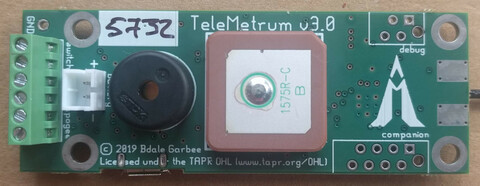
\includegraphics[width=\textwidth]{altusmetrum}
        \caption{Altus Metrum TeleMetrum~\cite{altus:telemetrum}.}
        \label{fig:altusmetrum}
    \end{subfigure}
    \hfill
    \begin{subfigure}[b]{0.48\textwidth}
        \centering
        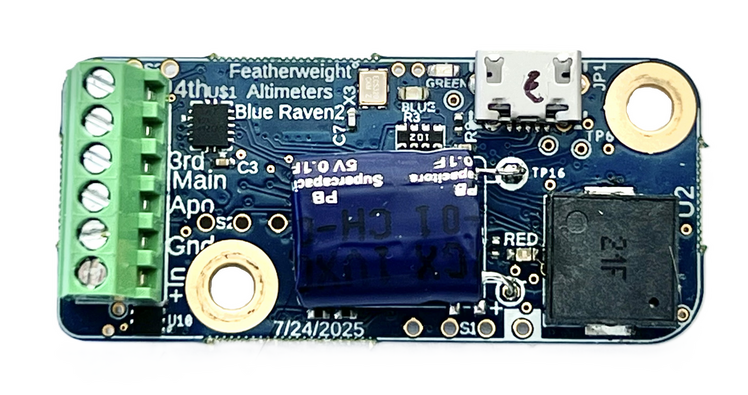
\includegraphics[width=\textwidth]{blueraven}
        \caption{Featherweight Blue Raven~\cite{featherweight:blueraven}.}
        \label{fig:blueraven}
    \end{subfigure}
    \caption{Examples of commercial flight computers for amateur rocketry.}
\end{figure}

Despite these advances, it is important to distinguish between systems primarily designed for altitude measurement and recovery, systems intended for flight-data transmission, and flight computers capable of estimating the vehicle's complete state in real time. The latter requires the integration of measurements from multiple sensors to reconstruct quantities such as attitude, position and velocity~\cite{ahrs,aiaa:rocketstateestimation}. Although these capabilities are well established in aerospace guidance and navigation systems, their implementation in compact, low-cost amateur rocket flight computers presents additional challenges in terms of computational resources, sensor integration and real-time operation.


% % % % % % % % % % % % % % % % % %
%                                 %
%  Master Thesis                  %
%  MSc in Aerospace Engineering   %
%  Mattia Gregnanin               %
%  A.Y. 2025/2026                 %
%                                 %
% % % % % % % % % % % % % % % % % %
%                                 %
%  Chapter 1 / Section 2          %
%                                 %
% % % % % % % % % % % % % % % % % %

\section{Components of a Flight Computer System}
\label{sec:components}

A flight computer for rockets typically consists of the functional blocks shown in \cref{fig:block_diagram}, which monitor and, in some cases, control the flight of the rocket. Each block is introduced in the following subsections in general terms, while the choices made for this work are discussed in \cref{sec:choices}.

\begin{figure}[htb]
    \centering
    \resizebox{\textwidth}{!}{%
    \begin{tikzpicture}[
        >={Latex[length=2mm]},
        block/.style={draw, rounded corners=2pt, minimum width=28mm, minimum height=9mm, align=center, font=\sffamily\small, drop shadow},
        sensor/.style={block, fill=blue!10},
        core/.style={block, thick, minimum width=34mm, minimum height=40mm, fill=red!20},
        output/.style={block, fill=green!10},
        ext/.style={block, dashed, minimum width=24mm, fill=yellow!10},
        pwr/.style={block, fill=orange!10}
    ]
    % Sensors
    \node[sensor] (imu)  at (-4.2, 1.65)  {IMU};
    \node[sensor] (mag)  at (-4.2, 0.55)  {Magnetometer};
    \node[sensor] (baro) at (-4.2,-0.55)  {Barometer};
    \node[sensor] (gnss) at (-4.2,-1.65)  {GNSS receiver};

    % Processing
    \node[core] (mcu) at (0,0) {Microcontroller\\[2mm] State estimation\\[2mm] Flight logic};

    % Outputs
    \node[output] (sd)    at (4.2, 1.4)  {Data storage\\(SD / flash)};
    \node[output] (radio) at (4.2, 0)    {Radio\\transceiver};
    \node[output] (pyro)  at (4.2,-1.4)  {Pyro channels\\(drivers)};

    % External elements
    \node[ext] (gs)      at (8.2, 0)    {Ground\\station};
    \node[ext] (charges) at (8.2,-1.4)  {Recovery\\charges};

    % Power
    \node[pwr] (pwr) at (0,-3.4) {Battery and power regulation};

    % Connections
    \foreach \s in {imu,mag,baro,gnss}
        \draw[->] (\s.east) -- (\s.east -| mcu.west);
    \draw[->]  (mcu.east |- sd.west)    -- (sd.west);
    \draw[<->] (mcu.east |- radio.west) -- (radio.west);
    \draw[->]  (mcu.east |- pyro.west)  -- (pyro.west);
    \draw[<->, dashed] (radio.east) -- node[above, font=\scriptsize]{RF link} (gs.west);
    \draw[->, dashed]  (pyro.east)  -- (charges.west);
    \draw[->]  (pwr.north) -- (mcu.south);
    \draw[->]  (pwr.west) -| (gnss.south);
    \draw[->]  (pwr.east) -| (pyro.south);
    \end{tikzpicture}}
    \caption{Block diagram of a typical flight computer of a rocket without active stabilization. Dashed elements are external to the board, while power connections to the remaining blocks are omitted for clarity.}
    \label{fig:block_diagram}
\end{figure}

\subsection{Microcontroller} 

Microcontrollers (MCUs) act as the central processing unit of the flight computer, responsible for gathering and processing data from the various sensors, writing data to storage, sending and receiving data from the communication modules, and executing the software that controls the rocket's flight. Common microcontrollers used in amateur rocketry include 8-bit devices such as the ATmega of Arduino boards, and 32-bit devices such as the ESP32 and the STM32 series. The 32-bit devices with a floating-point unit (FPU) are better suited to running state estimation algorithms onboard, which are demanding in terms of computation.
    
Some flight computers may even use multiple microcontrollers or microprocessors to handle different tasks, such as one for sensor data processing and another for communication and control~\cite{bps:ava}. This can improve the performance and reliability of the flight computer system by distributing the workload across multiple processing units, but requires careful design and coordination between the different microcontrollers to ensure an efficient and reliable operation of the overall system.

\subsection{Sensors} 

Flight computers are equipped with various sensors to measure different parameters during flight. Common sensors include:

\begin{itemize}
    \item \textbf{Accelerometers:} Measure the rocket's specific acceleration along multiple axes. Integrating it once and twice gives velocity and position, but the errors due to bias and noise grow linearly and quadratically with time, so inertial integration alone is accurate only over short intervals. When the non-gravitational acceleration is negligible, the direction of gravity also provides a reference for the orientation. Accelerometers with a wide measurement range (high-g) are used to measure shocks such as those of the ejection charges and of the landing. 
    \item \textbf{Gyroscopes:} Measure the rocket's angular velocity, helping to determine its orientation and stability during flight. Bias and noise produce errors that grow over time as the angular rate is integrated~\cite{titterton2004strapdown}. The combination of accelerometers and gyroscopes is often referred to as an \emph{Inertial Measurement Unit} (IMU).
    \item \textbf{Magnetometers:} Measure the Earth's magnetic field, which provides an absolute reference for the heading (the rotation about the vertical axis), not observable from accelerometers and gyroscopes alone. They are often subject to magnetic interference from the rocket's structure and electronics, thus requiring careful calibration and filtering to obtain accurate readings.
    \item \textbf{Barometers:} Measure atmospheric pressure, which can be used to calculate the altitude with a model of the atmosphere. The electronic bay of the rocket must be designed in order to allow ventilation, and the ground pressure must be measured before launch to provide a reference for altitude calculations.
    \item \textbf{GNSS Receivers:} Provide position and velocity at update rates typically between $\SIrange{1}{10}{Hz}$, and up to $\SI{25}{Hz}$ in some receivers~\cite{m9n:datasheet}, which allows the trajectory to be tracked and the rocket to be located after landing. Their performance depends on the antenna, on a clear view of the sky and on the dynamic model of the receiver, which may limit the acceleration, speed and altitude at which valid solutions are provided.
\end{itemize}

\subsection{Power Supply} 

Flight computers require a reliable power source throughout the flight. This is typically provided by batteries, with lithium polymer (LiPo) cells and alkaline batteries being used in amateur rocketry devices~\cite{altus:telemetrum,featherweight:blueraven}. The battery is chosen according to its capacity, weight, discharge current capability and voltage~\cite{reddy2011linden}. Since the battery voltage generally differs from the one required by the microcontroller and the sensors, and varies with the state of charge, it is converted to the appropriate levels using voltage regulators or power management circuits~\cite{horowitz2015art}.

Power distribution requires particular care in a rocket. Vibration and the high-current pulses drawn when a pyrotechnic igniter is fired can cause temporary voltage drops or momentary loss of electrical contact. If the supply voltage falls below the threshold of the microcontroller's \emph{brownout detector} (BOD), the device may reset, leading to a loss of flight data or of the recovery events. Two measures can be adopted to reduce this risk.

The first is power redundancy. Two batteries can be combined through Schottky diodes in an OR configuration: the load is supplied by the source with the higher voltage, and the diodes prevent one battery from supplying or discharging the other. Schottky diodes are preferred for their low forward voltage drop, which however still reduces the voltage available to the load and must be taken into account in the design~\cite{horowitz2015art}.

The second is the separation between the logic circuits (microcontroller and sensors) and the pyrotechnic channels. The igniters are driven by solid-state switches, such as power MOSFETs, while optoisolators can be used to transmit the control signal from the microcontroller to the driver without a direct electrical connection between the two circuits, so that current spikes and voltage sags on the pyrotechnic side do not propagate to the logic side~\cite{horowitz2015art}.

\subsection{Data Storage} 

Flight computers may include onboard data storage to log sensor and processed data during flight. Two types of non-volatile memory are commonly used:
\begin{itemize}
    \item \textbf{SD cards:} These removable storage devices offer high capacity and ease of use, allowing for quick data retrieval and analysis after the flight. However, they may be more susceptible to vibration and shock, corruption after sudden power loss, and they may break in the event of a hard landing.
    \item \textbf{Soldered flash memory:} Non-volatile memory chips that are soldered directly onto the flight computer's PCB. They are more robust and resistant to vibration and shock compared to SD cards, but they may have lower storage capacity and can be more difficult to access for data retrieval.
\end{itemize}

The telemetry link can be interrupted or limited in rate, so the onboard storage provides a complete record of the flight, which is used for post-flight analysis, for the validation of simulations and for reprocessing the estimation offline.

\subsection{Communication Modules}

A communication module allows the flight computer to exchange data with a ground station through a radio link. Its main function is the \emph{downlink} of telemetry, such as the estimated state, sensor readings and flight events, which allows the rocket to be monitored in real time and located after landing. A bidirectional \emph{transceiver} can also receive commands from the ground, for example for remote arming or configuration.

Flight computers for amateur rocketry use either the amateur radio bands, which require the user to hold a licence~\cite{altus:telemetrum}, or licence-exempt bands reserved for short-range devices (SRD). In Europe, the latter include the \SIrange{863}{870}{MHz} band, whose sub-bands are subject to limits on the radiated power and on the duty cycle~\cite{erc7003,etsi300220}. Common transceiver ICs, such as the Semtech SX127x family~\cite{sx1276}, support conventional frequency-shift keying (FSK) as well as the LoRa modulation, which trades data rate for receiver sensitivity and is therefore widely used for long-range, low-rate links~\cite{augustin2016lora}.

The performance of the link depends on the transmit power, the receiver sensitivity, the antennas and the environment, including the materials of the airframe.
    
\subsection{Recovery System Control}

Flight computers are commonly responsible for triggering the deployment of the recovery system, which slows the rocket down so that it can land safely. Deployment is usually achieved by igniting a small black powder charge that pressurizes a section of the airframe and separates it, releasing the parachute. The charge is ignited by an electric igniter (often called an \emph{e-match}), which is driven by a dedicated \emph{pyrotechnic channel} of the flight computer, typically a power transistor that briefly supplies a high current to the igniter~\cite{altus:telemetrum,featherweight:blueraven}. Alternatively, mechanical release mechanisms driven by servos or motors can be used.

The deployment events are decided from the measured flight conditions. The most common one is the detection of \emph{apogee}, i.e., the highest point of the trajectory, which is usually based on the barometric altitude and, in some devices, on accelerometer data~\cite{perfectflite,featherweight:blueraven}. A widely used scheme is \emph{dual deployment}, in which a small drogue parachute is released at apogee to limit the drift and the descent speed, and the main parachute is released at a lower, predefined altitude~\cite{altus:telemetrum}. This requires at least two independent pyrotechnic channels.

Since the channels handle pyrotechnic devices, safety measures are an integral part of the design. Typical examples are an arming switch that keeps the channels disconnected until shortly before launch, and a continuity check of the igniters, which verifies that they are correctly connected before flight~\cite{altus:telemetrum}.

\subsection{Actuators} 

Some rockets include active control systems, such as \emph{thrust vector control} (TVC), airbrakes to control the apogee, or movable fins and canards to control the roll. These systems use servomotors or other actuators commanded in closed loop from the estimated state of the rocket. The flight computer developed in this work does not include actuators: the estimated state is used for monitoring and for the recovery events only.

\subsection{Software} 

The software of a flight computer acquires the sensor measurements, estimates the state of the rocket, detects the flight events and manages data logging and telemetry. It is commonly organised around a fixed-rate main loop or a real-time operating system (RTOS) that schedules these tasks~\cite{white2024making}, with a \emph{finite state machine} (FSM) tracking the flight phases (liftoff, burnout, apogee, deployment, landing). The estimation algorithms and the firmware of this work are described in \cref{ch:estimation}.


% % % % % % % % % % % % % % % % % %
%                                 %
%  Master Thesis                  %
%  MSc in Aerospace Engineering   %
%  Mattia Gregnanin               %
%  A.Y. 2025/2026                 %
%                                 %
% % % % % % % % % % % % % % % % % %
%                                 %
%  Chapter 1 / Section 3          %
%                                 %
% % % % % % % % % % % % % % % % % %

\section{Existing Solutions}
\label{sec:existing}

This section reviews existing flight computers for amateur rocketry, covering both commercial products and open-source or student-developed projects. The solutions are compared according to the sensors they integrate, the pyrotechnic channels available for recovery, the state information they estimate, the telemetry capabilities and their openness. The review identifies which capabilities are widely available and which are less common, and provides the background for the design choices discussed in \cref{sec:choices}.

\subsection{Commercial Flight Computers}

Commercial flight computers for amateur rocketry can be grouped according to the sensors they integrate and the functions they provide. The boundaries between the groups are not sharp, since many manufacturers offer families of devices in which different models add sensors or telemetry to a common base. The main characteristics of the devices described below are summarised in \cref{tab:commercial-comparison}.

\paragraph{Recovery altimeters.} The simplest devices measure barometric altitude, log the flight and drive one or two pyrotechnic channels for recovery. After landing, they typically report the peak altitude to the user through a buzzer or an LED display. These devices are small, lightweight and relatively inexpensive, and for this reason they are also used as redundant recovery devices alongside a main flight computer. However, their functionality is limited to altitude-based events and basic data logging, and they do not estimate the full state of the rocket. Examples include the Altus Metrum EasyMini~\cite{altus:easymini}, the Altus Metrum TeleMini~\cite{altus:telemini}, which adds a radio link for telemetry, the PerfectFlite StratoLoggerCF~\cite{perfectflite}, the EggTimer Quark~\cite{eggtimer:quark} and the Jolly Logic AltimeterOne~\cite{jollylogic:altimeterone}, a logger without pyrotechnic channels that reports the altitude on an LED display.

\paragraph{Devices with inertial sensing.} These devices combine barometric altitude with inertial sensors, namely accelerometers and gyroscopes, which provide the acceleration and angular rate of the rocket in addition to its altitude. These measurements can be used, for example, to detect liftoff and burnout and to cross-check the barometric data. Wider measurement ranges, such as high-g accelerometers and gyroscopes with a high maximum angular rate, increase the cost of the device and are not necessary for every project. Examples include the Altus Metrum EasyMega~\cite{altus:easymega}, the Featherweight Blue Raven~\cite{featherweight:blueraven}, the EggTimer Proton~\cite{eggtimer:proton} and the Jolly Logic AltimeterTwo~\cite{jollylogic:altimetertwo}.

\paragraph{Devices with GNSS and telemetry.} The most complete devices add a GNSS receiver, and in most cases a radio transmitter, to the sensors described above. This allows the position of the rocket to be tracked in flight and recovered after landing, without relying on visual contact. The additional hardware increases the cost of the device, and, depending on the receiver, GNSS operation may be subject to limits on altitude and velocity, which are however not relevant for low-altitude flights.
Examples include the Altus Metrum TeleMetrum~\cite{altus:telemetrum}, the Altus Metrum TeleMega~\cite{altus:telemega} and the EggTimer Quasar~\cite{eggtimer:quasar}, which includes a built-in Wi-Fi module for data transmission.

\begin{table}[htbp]
    \centering
    \small
    \caption{Comparison of the commercial flight computers reviewed in this chapter. A tick means that the feature is available on the device.}
    \label{tab:commercial-comparison}
    \setlength{\tabcolsep}{4pt}
    \resizebox{\textwidth}{!}{%
    \begin{tabular}{llcccccccc}
        \toprule
        & \textbf{Device} & \textbf{Pyro ch.} & \textbf{Baro} & \textbf{Accel.} & \textbf{Gyro} & \textbf{Mag.} & \textbf{GNSS} & \textbf{Telemetry} & \textbf{Open source} \\
        \midrule
        \multicolumn{10}{l}{\emph{Recovery altimeters}} \\
        & Altus Metrum EasyMini  & 2 & \tick & \cross & \cross & \cross & \cross & \cross & \tick \\
        & Altus Metrum TeleMini  & 2 & \tick & \cross & \cross & \cross & \cross & \tick & \tick \\
        & PerfectFlite StratoLoggerCF & 2 & \tick & \cross & \cross & \cross & \cross & \cross & \cross \\
        & EggTimer Quark & 2 & \tick & \cross & \cross & \cross & \cross & \cross & \cross \\ 
        & Jolly Logic AltimeterOne & 0 & \tick & \cross & \cross & \cross & \cross & \cross & \cross \\
        \midrule
        \multicolumn{10}{l}{\emph{Inertial sensing}} \\
        & Altus Metrum EasyMega & 6 & \tick & \tick & \tick & \tick & \cross & \cross & \tick \\
        & Featherweight Blue Raven & 4 & \tick & \tick & \tick & \cross & \cross & \cross & \cross \\
        & EggTimer Proton & 6 & \tick & \tick & \tick & \cross & \cross & \cross & \cross \\
        & Jolly Logic AltimeterTwo & 0 & \tick & \tick & \cross & \cross & \cross & \cross & \cross \\
        \midrule
        \multicolumn{10}{l}{\emph{GNSS and telemetry}} \\
        & Altus Metrum Telemetrum & 2 & \tick & \tick & \cross & \cross & \tick & \tick & \tick \\
        & Altus Metrum TeleMega & 6 & \tick & \tick & \tick & \tick & \tick & \tick & \tick \\
        & EggTimer Quasar & 3 & \tick & \cross & \cross & \cross & \tick & \tick & \cross \\
        \bottomrule
    \end{tabular}}
\end{table}

\subsection{Open-Source and Student Projects}

Besides commercial products, a number of flight computers have been developed as open-source projects by hobbyists, student teams and companies supporting student rocketry. Their hardware designs and firmware are publicly available, which makes them a useful reference for the architectures and algorithms adopted in amateur rocketry. Unlike the commercial devices described above, most of them are documented mainly in project repositories and team websites rather than in the scientific literature.

The projects considered here were selected because their hardware, firmware or technical documentation is publicly available, and because they cover different levels of complexity, from the work of an individual hobbyist to that of student teams competing in international events. 
% Their main estimation and telemetry capabilities are compared in \cref{tab:open-source-comparison}.

\paragraph{CATS Vega.} The CATS Vega is an open-source flight computer for student rockets, developed by Control and Telemetry Systems GmbH and adopted as the official flight computer of the European Rocketry Challenge (EuRoC)~\cite{cats}.

It is based on an STM32F411 microcontroller and integrates an MS5607 barometric pressure sensor, a 6-axis IMU (LSM6DSO32) with an accelerometer of up to $\pm\SI{32}{\gforce}$ and a gyroscope of up to \SI{2000}{\degree\per\second}, a u-blox MAX-M10S GNSS receiver, a \SI{2.4}{GHz} LoRa transceiver and a flash memory that can store up to \SI{30}{min} of flight data~\cite{cats:vega}. The board is supplied with a voltage in the range \SIrange{7}{24}{V} and drives two pyrotechnic channels and two servo channels.

The Vega firmware is written in C++ using the PlatformIO framework and the Hardware Abstraction Layer (HAL) library provided by STMicroelectronics~\cite{cats:vegarepo}. A finite state machine (FSM) manages the flight phases, and each phase transition triggers a set of actions. The height above ground level, the vertical velocity and the bias of the measured vertical acceleration are estimated with a linear Kalman filter that fuses barometric and inertial measurements at a frequency of \SI{100}{Hz}~\cite{cats:vegaarticle}. The orientation of the rocket is estimated by integrating the angular rate measured by the gyroscope according to the quaternion kinematics equations~\cite{cats:vegarepo}. The telemetry module transmits the GNSS position and the estimated state at a frequency of \SI{10}{Hz}, and the data can be visualised in real time on the ground station~\cite{cats:vegaarticle}.

\begin{figure}[tb]
    \centering 
    \begin{subfigure}[b]{0.48\textwidth}
        \centering
        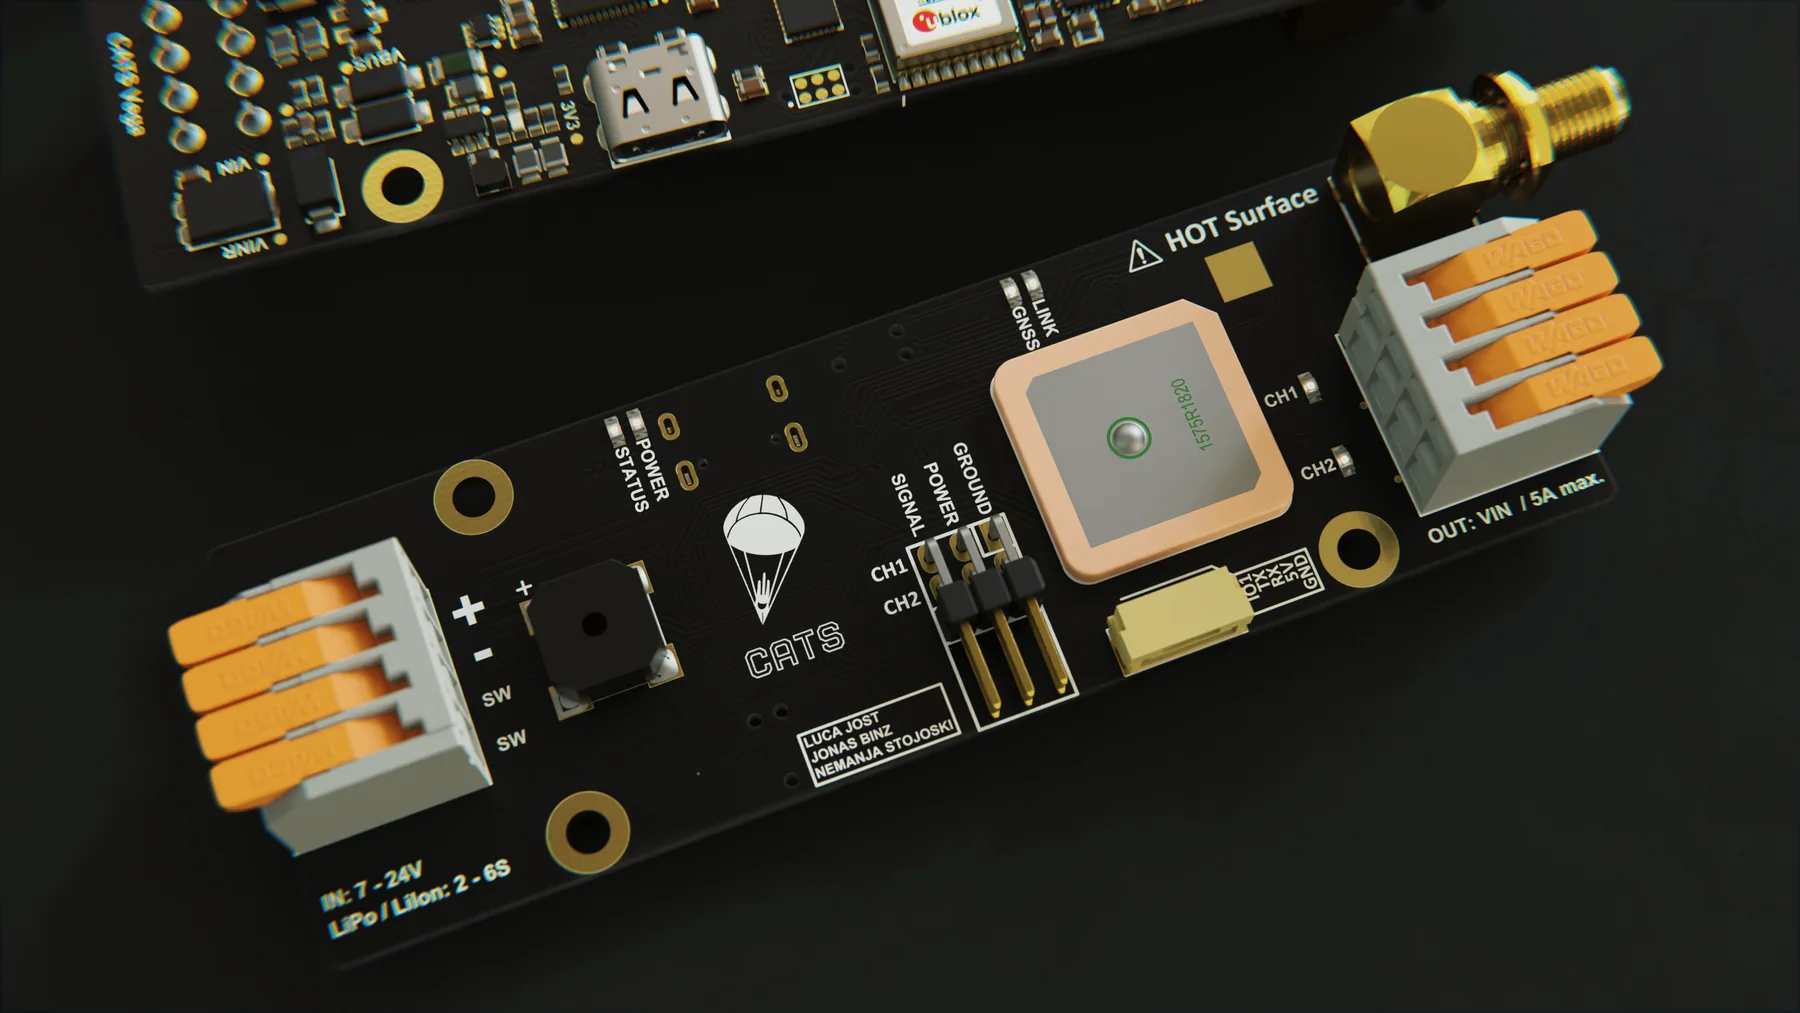
\includegraphics[width=\textwidth]{cats-vega}
        \caption{CATS Vega~\cite{cats:vega}.}
        \label{fig:cats-vega}
    \end{subfigure}
    \hfill
    \begin{subfigure}[b]{0.48\textwidth}
        \centering
        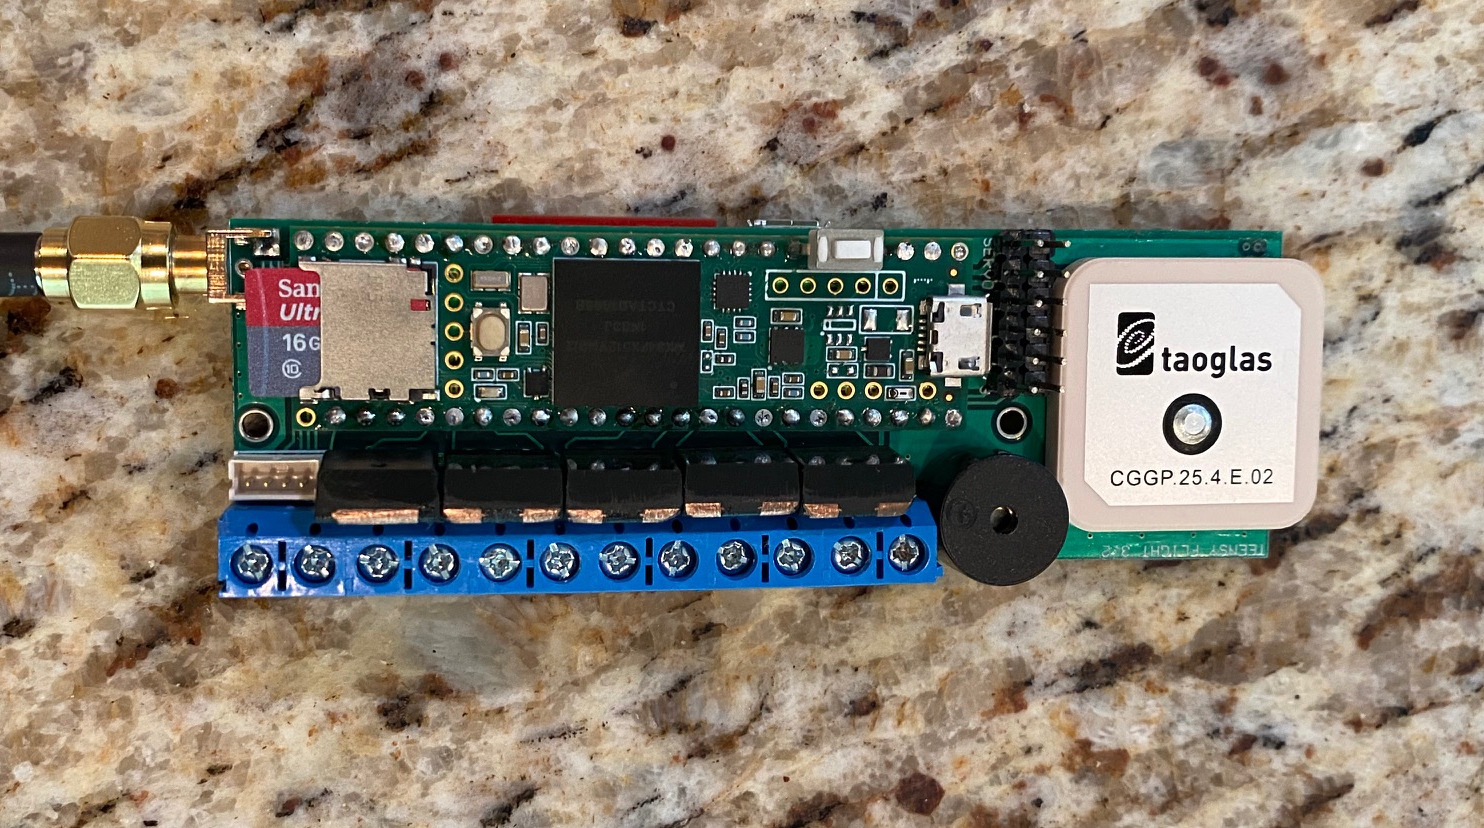
\includegraphics[width=\textwidth]{sparkyvt}
        \caption{HPR Rocket Flight Computer~\cite{sparkyvt:hpr-repo}.}
        \label{fig:sparkyvt}
    \end{subfigure}
    \caption{Open-source flight computers.}
    \label{fig:open-source-flight-computers}
\end{figure}


\paragraph{TUDSaT Zenith.} The Zenith is a flight computer developed by the RAPID student team of the Technical University of Darmstadt (TUDSaT) for their high-power hybrid rocket, which is expected to reach an apogee of $\SI{3}{km}$ at the EuRoC 2026 competition~\cite{tudsat:rapid}. % TODO: EuRoC 2026 takes place in October 2026. Verify the apogee after the competition 
The project is under active development, and the information reported here refers to the state of the repository at the time of writing~\cite{tudsat:zenithrepo}.

The board is based on an STM32H743 microcontroller and integrates redundant sensors: three barometric pressure sensors (MS5607, BMP580 and LPS22HB), three 6-axis IMUs (ICM-42670-P, ICM-42688-P and LSM6DSO32), a high-g accelerometer (H3LIS331DL), a magnetometer (LIS3MDL), a u-blox GNSS receiver, a W25Q SPI flash memory and a \SI{868}{MHz} LoRa transceiver~\cite{tudsat:zenithrepo}.

The firmware is written in Rust and uses the Embassy framework for embedded systems. A finite state machine (FSM) manages the flight phases, and the state of the rocket is estimated by combining two filters: a Mahony filter for the orientation and a 9-dimensional linear Kalman filter for the position, velocity and acceleration~\cite{tudsat:zenithrepo}.
The estimation runs at a frequency of \SI{1000}{Hz}~\cite{tudsat:zenithrepo}.

\paragraph{HPR Rocket Flight Computer.} The HPR Rocket Flight Computer is an open-source flight computer developed by an individual hobbyist, SparkyVT, for high-power rocketry~\cite{sparkyvt:hpr-repo}.

The board can be customised by the user: it is compatible with different microcontrollers of the Teensy family and can integrate different kinds of sensors. The default configuration includes a Teensy 4.1 microcontroller, an MS5611 barometric pressure sensors, an LSM6DSOX 6-axis IMU, an H3LIS331DL high-g accelerometer, a u-blox NEO-M9N GNSS receiver and an RFM96W or RFM95W LoRa transceiver, which can operate, respectively, in the \SI{433}{MHz} and \SI{868}{MHz} bands. The board can drive four pyrotechnic channels and eight servo channels.

The firmware is written in C++ using the Arduino framework. The altitude and the vertical velocity are estimated with a complementary filter that fuses barometric and inertial measurements at a frequency of ì\SI{1000}{Hz}. 
The orientation of the rocket is estimated by integrating the angular rate measured by the gyroscope according to the quaternion kinematics equations at a frequency of \SI{100}{Hz}.
The telemetry module transmits the GNSS position and the estimated state at a frequency of \SI{20}{Hz}, and the data can be visualised in real time on the ground station~\cite{sparkyvt:hpr-repo}. 

\paragraph{Vector II.} The Vector II is a sounding rocket developed by the State University of Londrina (UEL), Brazil, for educational and research purposes~\cite{NETZEL2026e00803}.

Its flight computer is based on an STM32F407 microcontroller and integrates an MS5607 barometric pressure sensor, an ICM-42670-P 6-axis IMU, an ADXL375 high-g accelerometer, an MMC5983MA magnetometer and a \SI{64}{Mbit} flash memory. It drives two pyrotechnic channels for the recovery system, which are fired once the apogee is detected.

The firmware uses the STMicroelectronics HAL library and implements a finite state machine (FSM) to manage the flight phases. The raw sensor measurements are stored in the flash memory at a frequency of \SI{12.5}{Hz}. The apogee is detected when the barometric pressure starts to increase monotonically~\cite{NETZEL2026e00803}. The system does not include a radio link and relies on post-flight analysis of the logged data.

% \begin{table}[htbp]
%     \centering
%     \small
%     \setlength{\tabcolsep}{4pt}
%     \caption{Estimation and telemetry capabilities of the open-source and student projects reviewed in this chapter.}
%     \label{tab:open-source-comparison}
%     \resizebox{\textwidth}{!}{%
%     \begin{tabular}{lcccc}
%         \toprule
%         \textbf{Project} & \textbf{MCU} & \textbf{Orientation est.} & \textbf{Position/velocity est.} & \textbf{Telemetry} \\
%         \midrule
%         CATS Vega & STM32F411 & Gyro integration & Vertical Kalman filter & LoRa, $\SI{2.4}{GHz}$ \\
%         TUDSaT Zenith & STM32H743 & Mahony filter & 9-state Kalman filter & LoRa, $\SI{868}{MHz}$ \\
%         HPR & Teensy 4.1 & Gyro integration & Complementary filter (vertical) & LoRa, 433/\SI{868}{MHz} \\
%         Vector II & STM32F407 & \cross & \cross & \cross \\
%         \bottomrule
%     \end{tabular}}
% \end{table}

\subsection{Summary and Open Issues}

Overall, the solutions reviewed in this section fall into two groups. Commercial flight computers are mature and well documented, and they are designed primarily around recovery and flight logging: barometric altitude and, in some models, inertial measurements are used to detect flight events, while GNSS receivers and telemetry are available only on the more complete devices. In the documentation reviewed, none of them provides an estimate of the full state of the rocket, and, with the exception of the Altus Metrum products, their hardware and firmware are not open. 

Open-source and student projects are more diverse. The CATS Vega and the TUDSaT Zenith combine onboard state estimation with a LoRa downlink, whereas the HPR Rocket Flight Computer estimates only the vertical channel and the Vector II logs the raw measurements without estimating the state or transmitting it. Among the projects considered, the orientation is obtained in most cases by integrating the angular rate of the gyroscope, which does not correct the drift of the estimate, and only the Zenith applies a dedicated attitude filter. Moreover, the design choices and the estimation algorithms are mostly documented in repositories and team websites rather than in peer-reviewed publications, which makes it difficult to compare them or to reproduce them.

To the best of our knowledge, no solution among those reviewed combines all of the following: a complete estimate of attitude, position and velocity based on sensor fusion, a telemetry link in a licence-exempt band suitable for European regulations, and a design simple and documented enough to be reproduced by a small team. This is the space addressed by this work, whose design choices are motivated in the next section.


% % % % % % % % % % % % % % % % % %
%                                 %
%  Master Thesis                  %
%  MSc in Aerospace Engineering   %
%  Mattia Gregnanin               %
%  A.Y. 2025/2026                 %
%                                 %
% % % % % % % % % % % % % % % % % %
%                                 %
%  Chapter 1 / Section 4          %
%                                 %
% % % % % % % % % % % % % % % % % %

\newcommand{\reqdef}[1]{\hypertarget{req:#1}{#1}}
\newcommand{\req}[1]{\hyperlink{req:#1}{#1}}

\section{Design Choices}
\label{sec:choices}

The review in \cref{sec:existing} shows that most flight computers for amateur rocketry are designed around recovery and flight logging, and that the few solutions providing onboard state estimation and telemetry differ in the quantities they estimate and in the documentation available.

Starting from this background, this section defines the requirements of the flight computer developed in this work and motivates the choice of each of its components. The requirements are presented first, and are then used as criteria to compare the alternatives found in the existing solutions and to justify the selected components. The hardware implementation of the selected components is described in Chapter~\ref{ch:hardware}.

\subsection{Requirements}
\label{sec:requirements}

The flight computer is intended for an amateur rocket developed by a small team of students, with a target apogee of about $\SI{500}{m}$ in the current configuration (class F motor) and the possibility of reaching higher altitudes in future versions. Its objective is to measure the flight with onboard sensors, to reconstruct the attitude, position and velocity of the rocket and to transmit them to a ground station by radio. The following requirements were derived from this objective and from the limitations of the solutions reviewed in Section~\ref{sec:existing}.

The requirements of the flight computer are divided into functional requirements (\cref{tab:functional-requirements}), which describe what the system must do, performance requirements (\cref{tab:performance-requirements}), which quantify how well it must do it, and constraints (\cref{tab:design-requirements}), which limit the design space. 

\begin{table}[tbp]
    \centering
    \small
    \renewcommand{\arraystretch}{1.25}
    \caption{Functional requirements. Verification methods: T = test, A = analysis, I = inspection, D = demonstration.}
    \label{tab:functional-requirements}
    \begin{tabularx}{\textwidth}{@{}l >{\raggedright\arraybackslash}X >{\raggedright\arraybackslash}X c@{}}
        \toprule
        \textbf{ID} & \textbf{Requirement} & \textbf{Rationale} & \textbf{Verif.} \\
        \midrule
        \reqdef{F01} & The system shall acquire measurements from the onboard sensors. & Input of the estimation algorithm and data for post-flight analysis. & T \\
        \reqdef{F02} & The system shall estimate the attitude, position and velocity of the rocket onboard. & Core objective of the work. & T, A \\
        \reqdef{F03} & The system shall detect the flight events and trigger the corresponding actions. & Safe recovery of the rocket or active guidance. & T, D \\
        \reqdef{F04} & The system shall transmit the estimated state and the GNSS position to a ground station. & Real-time monitoring and recovery of the rocket. & T \\
        \reqdef{F05} & The system shall store flight data in non-volatile memory. & Post-flight analysis and validation of the estimation algorithm. & T, I \\
        \reqdef{F06} & The system shall provide two pyrotechnic channels to control the recovery system. & Safe recovery of the rocket. & T, D \\
        \bottomrule
    \end{tabularx}
\end{table}

\begin{table}[tbp]
    \centering
    \small
    \renewcommand{\arraystretch}{1.25}
    \caption{Performance requirements. Each requirement refers to the functional requirement it quantifies. Verification methods: T = test, A = analysis, I = inspection.}
    \label{tab:performance-requirements}
    \begin{tabularx}{\textwidth}{@{}l >{\raggedright\arraybackslash}X >{\raggedright\arraybackslash}X c@{}}
        \toprule
        \textbf{ID} & \textbf{Requirement} & \textbf{Acceptance criterion} & \textbf{Verif.} \\
        \midrule
        \reqdef{P01.01} & Sensor sampling rate of at least \SI{100}{Hz}. & Measured sampling period within \SI{1}{\percent} of nominal. & T \\
        \reqdef{P01.02} & GNSS receiver sampling rate of at least \SI{1}{Hz}. & Measured sampling period within \SI{1}{\percent} of nominal. & T \\
        \midrule
        \reqdef{P02.01} & State estimation update rate of at least \SI{100}{Hz}. & Measured update period within \SI{1}{\percent} of nominal. & T \\
        \reqdef{P02.02} & Attitude estimation error below \SI{5}{\degree}. & Comparison with a reference (simulation or ground-truth flight) on the same data. & T, A \\
        \reqdef{P02.03} & Position estimation error below \SI{10}{m}. & Comparison with a reference (simulation or ground-truth flight) on the same data. & T, A \\
        \reqdef{P02.04} & Velocity estimation error below \SI{5}{m/s}. & Comparison with a reference (simulation or ground-truth flight) on the same data. & T, A \\
        \midrule
        \reqdef{P03.01} & Flight event detection latency within \SI{0.1}{s}. & Measured latency on a reference flight. & T \\
        \reqdef{P03.02} & Apogee detection error below \SI{10}{m}. & Comparison with a reference (simulation or ground-truth flight) on the same data. & T, A \\
        \midrule
        \reqdef{P04.01} & Telemetry link range of at least \SI{1}{km}. & Measured range in a line-of-sight test. & T \\
        \reqdef{P04.02} & Telemetry link data rate of at least \SI{2.4}{kbps}. & Measured data rate in a line-of-sight test. & T \\
        \midrule
        \reqdef{P05.01} & Data storage capacity of at least \SI{30}{minutes} of flight data. & Measured available storage space. & I \\
        \midrule
        \reqdef{P06.01} & The pyrotechnic channels must be able to drive a load with a nominal resistance of \SI{1.5}{\ohm} at a current of at least \SI{0.4}{A}. & Measured current and voltage on a resistive load. & T \\
        \bottomrule 
    \end{tabularx}
\end{table}

\begin{table}[tbp]
    \centering
    \small
    \renewcommand{\arraystretch}{1.25}
    \caption{Design requirements. Verification methods: T = test, A = analysis, I = inspection.}
    \label{tab:design-requirements}
    \begin{tabularx}{\textwidth}{@{}l >{\raggedright\arraybackslash}X >{\raggedright\arraybackslash}X c@{}}
        \toprule
        \textbf{ID} & \textbf{Requirement} & \textbf{Rationale} & \textbf{Verif.} \\
        \midrule
        \reqdef{D01} & The board must fit in an electronics bay of at most \SI{50}{mm} diameter and \SI{80}{mm} length. & Airframe design. & I \\
        \reqdef{D02} & The system must withstand an acceleration of up to \SI{100}{\gforce} and must not reset when the pyrotechnic channels are fired. & Lift-off and recovery events. & T \\
        \reqdef{D03} & The system must operate in a temperature range of at least \SIrange{-20}{50}{\degreeCelsius} and up to \SI{10}{km} of altitude. & Flight environment. & T \\
        \reqdef{D04} & The board must be powered by a single \SI{3.7}{V} LiPo battery. & Simplicity and availability of the power source. & I \\
        \reqdef{D05} & The cost of the components must not exceed about 100 \texteuro{} per board. & Affordability for a amateur team. & I \\
        \reqdef{D06} & The radio link must operate in a licence-exempt band. & Regulatory compliance. & A, T \\
        \reqdef{D07} & The pyrotechnic channels shall remain disabled until the rocket is armed. & Safety rules~\cite{nar:safetycode,tripoli:safetycode}. & T, I \\
        \bottomrule
    \end{tabularx}
\end{table}

\subsection{Microcontroller}
\label{sec:mcu-choice}

\paragraph{Requirements.} The microcontroller shall satisfy the following requirements, which derive from the functional and performance requirements of \cref{tab:functional-requirements,tab:performance-requirements,tab:design-requirements}:
\begin{itemize}
    \item a single-precision floating-point unit (FPU) and a computing power sufficient to run the estimation algorithm at the required rate with an adequate margin (\req{P02.01}); 
    \item at least 3 SPI, 3 I\textsuperscript{2}C and 2 UART interfaces to connect the sensors, the GNSS receiver, the radio module and the storage (\req{F01}, \req{F04}, \req{F05});
    \item enough RAM for the state and covariance matrices of the filter and for the data buffers, and enough flash memory for the firmware; % TODO: give an estimate of the memory needed
    \item a USB interface and a hardware debug interface (SWD or JTAG) for programming, data download and debugging;
    \item a low cost and a long-term availability, supported by a wide community and by manufacturer documentation (\req{D05}). % TODO: give a target cost
\end{itemize}

\paragraph{Alternatives.} The microcontrollers used by the solutions reviewed in \cref{sec:existing} are listed in \cref{tab:mcu-comparison}. Hobbyist designs often rely on 8-bit microcontrollers such as the ATmega, which lack an FPU and have limited memory, and are therefore not adequate for the estimation algorithm. Among 32-bit devices, the ESP32 family offers a high clock frequency at low cost, and integrates Wi-Fi and Bluetooth, which are not needed in this application. The STM32 family offers a wide range of devices based on ARM Cortex-M cores with FPU, from the STM32F4 series (Cortex-M4, up to $\SI{180}{MHz}$) to the STM32H7 series (Cortex-M7, up to $\SI{480}{MHz}$ or more depending on the device), and is used by three of the four open-source projects reviewed. The Teensy 4.1 used in the HPR flight computer offers a much higher computing power, but it is a development board and not a bare microcontroller.

\begin{table}[htb]
    \centering
    \small
    \caption{Microcontrollers of the flight computers reviewed in Section~\ref{sec:existing} and of the main alternatives.}
    \label{tab:mcu-comparison}
    \begin{tabular}{@{}l l c c c l@{}}
        \toprule
        \textbf{MCU} & \textbf{Core} & \textbf{Clock} & \textbf{RAM} & \textbf{Flash} & \textbf{Used in} \\
        & & {\footnotesize (\unit{\mega\hertz})} & {\footnotesize (\unit{\kilo\byte})} & {\footnotesize (\unit{\mega\byte})} & \\
        \midrule
        STM32F411 & Cortex-M4F & 100 & 128 & 0.5 & Vega \\
        STM32F407 & Cortex-M4F & 168 & 192 & 1 & Vector II \\
        STM32F405 & Cortex-M4F & 168 & 192 & 1 & This work \\
        STM32H743 & Cortex-M7 & 480 & 1024 & 2 & TUDSaT Zenith \\
        Teensy 4.1 & Cortex-M7 & 600 & 1024 & 8 & HPR \\
        ESP32 & Xtensa LX6 (dual) & 240 & 520 & external & -- \\
        \bottomrule
    \end{tabular}
\end{table}

\paragraph{Choice.} The STM32F405RGT6 was selected, in the LQFP64 package~\cite{stm32f405:datasheet}. It has a Cortex-M4 core with a single-precision FPU running at up to \SI{168}{MHz}, \SI{192}{kB} of SRAM and \SI{1}{MB} of flash memory, and provides 3 SPI, 3 I\textsuperscript{2}C and 6 UART interfaces, USB and SWD, which satisfy the requirements above.
The estimation filter requires about [X] kB of RAM and an execution time of [Y]\,\textmu s per update, which corresponds to a CPU load of about [Z]\,\% at the update rate of $\SI{1}{Hz}$. % TODO: replace with a measurement or an estimate: this is the most important justification
The STM32F4 series was preferred to the ESP32 for the development environment and the availability of development tools. A higher-end device such as the STM32H743 was not necessary, since the F405 already provides an adequate margin for the algorithm, and it is the same family used by the Vector II (F407)~\cite{NETZEL2026e00803} with similar characteristics.

\subsection{Inertial Measurement Unit}
\label{sec:imu-choice}

\paragraph{Requirements.} The inertial measurement unit (IMU) shall satisfy the following requirements:
\begin{itemize}
    \item a 3-axis accelerometer and a 3-axis gyroscope, with a measurement range covering the maximum acceleration and angular rate expected during the flight, of at least $\pm\SI{16}{\gforce}$ and $\pm\SI{2000}{\degree/s}$ respectively (\req{F01});
    \item an output data rate of at least \SI{100}{Hz} (\req{P01.01});
    \item a noise density and a bias stability sufficient to keep the attitude, velocity and position errors within the limits of \req{P02.02}, \req{P02.03} and \req{P02.04};
    \item a low cost and good availability (\req{D05}).
\end{itemize}

\paragraph{Alternatives.} The IMUs adopted by the open-source flight computers reviewed in \cref{sec:existing}, together with two widely used devices, are compared in \cref{tab:imu-comparison}. The MPU-6050 has long been the reference IMU of hobbyist projects thanks to its low cost and wide software support, but it has a higher noise density than the more recent devices and the manufacturer does not recommend it for new designs~\cite{mpu6050:datasheet}. Among the devices used in the reviewed projects, the ICM-42688-P and the LSM6DSO32 offer respectively a low noise density and an extended accelerometer range of $\pm\SI{32}{\gforce}$, but not both. In the reviewed projects, a wide range is obtained either with an IMU with a high accelerometer full-scale (CATS Vega) or by adding a separate high-g accelerometer (TUDSaT Zenith, HPR and Vector II).

\begin{table}[htb]
    \centering
    \small
    \setlength{\tabcolsep}{3pt}
    \caption{Comparison of the IMUs used in the flight computers reviewed in \cref{sec:existing} and of the main alternatives. The resolution is the maximum available at the indicated full scale, and the noise density is given in the low-noise mode.}
    \label{tab:imu-comparison}
    \begin{tabular}{@{}l ccc ccc l@{}}
        \toprule
        & \multicolumn{3}{c}{\textbf{Accelerometer}} & \multicolumn{3}{c}{\textbf{Gyroscope}} & \\
        \cmidrule(lr){2-4} \cmidrule(lr){5-7}
        \textbf{IMU} & \textbf{Range} & \textbf{Res.} & \textbf{Noise} & \textbf{Range} & \textbf{Res.} & \textbf{Noise} & \textbf{Used in} \\
        & {\scriptsize (\unit{\gforce})} & {\scriptsize (\unit{\lsb/\gforce})} & {\scriptsize (\unit{\micro\gforce/\rthz})} & {\scriptsize (\unit{\degree/\second})} & {\scriptsize (\unit{\lsb\per(\degree\per\second)})} & {\scriptsize (\unit{(\milli\degree\per\second)\per\rthz})} & \\
        \midrule
        MPU-6050~\cite{mpu6050:datasheet}     & $\pm16$ & 2048 & 400 & $\pm2000$ & 16.4 & 5 & -- \\
        BMI088~\cite{bmi088:datasheet}        & $\pm24$ & 1365 & \numrange{160}{190} & $\pm2000$ & 16.4 & 14 & -- \\
        ICM-42670-P~\cite{icm42670:datasheet} & $\pm16$ & 2048 & 100 & $\pm2000$ & 16.4 & 7 & Zenith, Vector II \\
        ICM-42688-P~\cite{icm42688:datasheet} & $\pm16$ & 8192 & \numrange{65}{75} & $\pm2000$ & 131 & 2.8 & Zenith \\
        ICM-45686~\cite{icm45686:datasheet} & $\pm32$ & 16384 & 110 & $\pm4000$ & 131 & 3.8 & This work \\
        LSM6DSOX~\cite{lsm6dsox:datasheet}    & $\pm16$ & 2048 & 110 & $\pm2000$ & 14.3 & 3.8 & HPR \\
        LSM6DSO32~\cite{lsm6dso32:datasheet}  & $\pm32$ & 1024 & 220 & $\pm2000$ & 14.3 & 3.8 & Vega, Zenith \\
        \bottomrule
    \end{tabular}
\end{table}

\paragraph{Choice.} The ICM-45686 was selected~\cite{icm45686:datasheet}. Its main advantage is that it provides a wide accelerometer range of $\pm\SI{32}{\gforce}$ without losing resolution: the data can be read in a 20-bit format, which corresponds to \SI{16384}{\lsb/\gforce}, while a 16-bit device with the same full scale, such as the LSM6DSO32, has a resolution of about \SI{1}{m\gforce}, comparable to the noise of the sensor over a bandwidth of \SI{100}{Hz}. The wide range makes a separate high-g accelerometer necessary only for high power rockets. The gyroscope range of $\pm\SI{4000}{\degree/\second}$ exceeds the requirement of \req{F01} and provides a margin for the roll rate of the rocket. Its noise density, \SI{110}{\micro\gforce/\rthz} for the accelerometer and \SI{3.8}{(\milli\degree\per\second)\per\sqrt{\Hz}} for the gyroscope, is comparable to the other devices with the same range. The sensor communicates over an SPI interface at up to \SI{24}{MHz}, compatible with the interfaces of the microcontroller (\cref{sec:mcu-choice}). Drawbacks are its short history, which means fewer reference implementations than the ICM-42xxx or LSM6DS families, and its cost and availability.

\subsection{High-g Accelerometer}
\label{sec:high-g-choice}

\paragraph{Requirements.} In addition to the IMU described in \cref{sec:imu-choice}, whose accelerometer range is $\pm\SI{32}{\gforce}$, the flight computer includes a separate high-g accelerometer to capture the shocks that occur during the recovery sequence and the landing, namely the firing of the ejection charges, the opening of the parachutes and the impact with the ground, which may exceed the range of the IMU and last only a few milliseconds. The high-g accelerometer shall satisfy the following requirements:
\begin{itemize}
    \item a measurement range of at least $\pm\SI{100}{\gforce}$, to capture the peak acceleration of these events (\req{D02});
    \item an output data rate of at least \SI{1000}{Hz}, high enough to sample shocks lasting a few milliseconds without aliasing;
    \item a bias and a noise level compatible with the detection and the recording of the events, which are the only uses of this sensor;
    \item a low cost and good availability (\req{D05}).
\end{itemize}

\paragraph{Alternatives.} The simplest alternative is to rely only on the IMU, as the CATS Vega does, with the risk of saturating the sensor during the shocks. The separate high-g accelerometers used by the reviewed projects are compared in \cref{tab:high-g-comparison}: the ADXL375 in the Vector II and the H3LIS331DL in the TUDSaT Zenith and in the HPR flight computer. The H3LIS331DL has selectable ranges of $\pm\SI{100}{\gforce}$, $\pm\SI{200}{\gforce}$ and $\pm\SI{400}{\gforce}$, and is compared with the ADXL375 at $\pm\SI{200}{\gforce}$.

\begin{table}[htb]
    \centering
    \small
    \caption{Comparison of the high-g accelerometers used in the flight computers reviewed in \cref{sec:existing}, at the same range of $\pm\SI{200}{\gforce}$.}
    \label{tab:high-g-comparison}
    \begin{tabular}{@{}lccccl@{}}
        \toprule
        \textbf{Model} & \textbf{Res.} & \textbf{ODR} & \textbf{Noise} & \textbf{0\,\unit{\gforce} offset} & \textbf{Used in} \\
        & {\footnotesize (\unit{\lsb/\gforce})} & {\footnotesize (\unit{\hertz})} & {\footnotesize (\unit{\milli\gforce/\rthz})} & {\footnotesize (\unit{\milli\gforce})} & \\
        \midrule
        ADXL375~\cite{adxl375:datasheet} & 20.5 & 3200 & 5 & $\pm400$ & Vector II, this work \\
        ADXL372~\cite{adxl372:datasheet} & 10 & 6400 & -- & $\pm1000$ & -- \\
        H3LIS331DL~\cite{h3lis331dl:datasheet} & 10.2 & 1000 & 15 & $\pm1000$ & Zenith, HPR \\
        \bottomrule
    \end{tabular}
\end{table}

\paragraph{Choice.} The ADXL375 was selected~\cite{adxl375:datasheet}. Its fixed range of $\pm\SI{200}{\gforce}$ covers the expected shocks with margin, and its output data rate of up to \SI{3200}{Hz} is high enough to sample them. Its resolution of about \SI{49}{\milli\gforce} per LSB and its noise density are much worse than those of the IMU, and the zero-g offset is large, so the sensor is used only to detect and record the shocks and not for the estimation of attitude, velocity and position, which rely on the accelerometer of the IMU.

\subsection{Magnetometer}
\label{sec:mag-choice}

\paragraph{Requirements.} A magnetometer provides an absolute reference for rotation through the Earth's magnetic field, whose intensity is about \SI{48}{\micro\tesla} in Nothern Italy. The magnetometer shall satisfy the following requirements:
\begin{itemize}
    \item a 3-axis measurement with a range of at least $\pm\SI{250}{\micro\tesla}$, which covers the Earth's field and the disturbances generated by the electronics of the rocket, such as the current of the pyrotechnic channels, which can reach hundreds of microtesla at a distance of a few millimeters from the board (\req{F01});
    \item a noise level and a calibration capability that keep the heading error below the limit of \req{P02.02}; 
    \item an output data rate compatible with the update rate of the heading correction in the estimation filter (\req{P01.01}); 
    \item a low cost and good availability (\req{D05}).
\end{itemize}

\paragraph{Alternatives.} The simplest alternative is to omit the magnetometer and estimate the attitude by integrating only the angular rate, as the CATS Vega and the HPR flight computer do (\cref{sec:existing}), at the cost of an unbounded drift of the heading and zero knowledge of the absolute orientation. The magnetometers adopted by the reviewed projects are compared in \cref{tab:mag-comparison}: the LIS3MDL in the TUDSaT Zenith and the MMC5983MA in the Vector II, which however does not estimate the attitude onboard. The MMC5983MA has a lower noise level and a higher output data rate, and provides a SET/RESET function that allows the offset to be measured and removed~\cite{mmc5983ma:datasheet}. The LIS3MDL is no longer recommended for new designs by the manufacturer~\cite{lis3mdl:page}.

\begin{table}[htb]
    \centering
    \small
    \caption{Comparison of the magnetometers used by the flight computers reviewed in \cref{sec:existing} and of the one adopted in this work. ODR is the output data rate. The resolution is the maximum available at the indicated full scale, and the noise is the RMS value in the highest-performance mode.
    }
    \label{tab:mag-comparison}
    \begin{tabular}{@{}lccccl@{}}
        \toprule
        \textbf{Model} & \textbf{Range} & \textbf{Res.} & \textbf{ODR} & \textbf{Noise (RMS)} & \textbf{Used in} \\
        & {\footnotesize (\unit{\micro\tesla})} & {\footnotesize (\unit{\nano\tesla/\lsb})} & {\footnotesize (\unit{\hertz})} & {\footnotesize (\unit{\nano\tesla})} & \\
        \midrule
        LIS3MDL~\cite{lis3mdl:datasheet} & $\pm1600$ & 58.5 & 150 & \numrange{320}{410} & Zenith \\
        MMC5983MA~\cite{mmc5983ma:datasheet} & $\pm800$ & 6.1 & 1000 & 120 & Vector II \\
        LIS2MDL~\cite{lis2mdl:datasheet} & $\pm4915$ & 150 & 100 & 300 & This work \\
        \bottomrule
    \end{tabular}
\end{table}

\paragraph{Choice.} The LIS2MDL was selected~\cite{lis2mdl:datasheet}. Its noise of about $\SI{300}{nT}$ corresponds to a heading error of about $\SI{0.8}{\degree}$ (1$\sigma$) for a horizontal field of $\SI{22}{\micro\tesla}$, which is small compared to the errors due to the hard-iron and soft-iron disturbances of the rocket, so that the lower noise of the MMC5983MA would not improve the estimate significantly. Its range of $\pm\SI{4915}{\micro\tesla}$ avoids saturation in the presence of local disturbances, with no loss of resolution, which is fixed at \SI{150}{\nano\tesla} per LSB. The sensor is placed far from the the pyrotechnic lines and the servo motors. It communicates over an I\textsuperscript{2}C interface at up to \SI{400}{kHz}, compatible with the interfaces of the microcontroller (\cref{sec:mcu-choice}). Its main disadvantage compared with the MMC5983MA is the lower output data rate, which however is sufficient for the correction step of the filter, and the absence of a degaussing function.

\subsection{Barometer}
\label{sec:baro-choice}

\paragraph{Requirements.} A barometer measures the atmospheric pressure, from which the altitude of the rocket is obtained with a model of the atmosphere, and provides the absolute altitude reference used to correct the drift of the inertial integration. The barometer shall satisfy the following requirements:
\begin{itemize}
    \item a measurement range covering the pressure at the launch site and the pressure at the maximum altitude considered for the design, which is about \SI{265}{hPa} at \SI{10}{km} in the standard atmosphere~\cite{iso2533} (\req{D02});
    \item a pressure noise corresponding to an altitude noise below the limits of \req{P02.03} and \req{P03.02}, in the configuration used in flight;
    \item an output data rate compatible with the update rate of the altitude correction in the estimation filter (\req{P01.01});
    \item a low cost and good availability (\req{D05}).
\end{itemize}
The altitude noise corresponding to a given pressure noise grows with altitude, because the air density decreases: \SI{1}{Pa} corresponds to about \SI{8}{cm} near sea level and to about \SI{25}{cm} at \SI{10}{km}.

\paragraph{Alternatives.} The barometers adopted by the reviewed projects are compared in \cref{tab:baro-comparison}: the MS5607 is used by the CATS Vega, the TUDSaT Zenith and the Vector II, the MS5611 by the HPR flight computer, and the BMP580 and the LPS22HB by the Zenith, which uses three barometers for redundancy. The MS5611 has the same pressure range at low pressure as the MS5607 and a lower noise, and the two devices share the same interface~\cite{ms5611:datasheet,ms5607:datasheet}. The BMP580 has a noise about one order of magnitude lower, but its minimum pressure of about \SI{300}{hPa} limits the maximum altitude to about \SI{9}{km} in the standard atmosphere~\cite{bmp580:datasheet}. The maximum output data rate of the LPS22HB is about \SI{75}{Hz}~\cite{lps22hb:datasheet}, which is sufficient only if the rate required by the filter is lower. 

\begin{table}[htb]
    \centering
    \small
    \caption{Comparison of the barometers of the flight computers reviewed in \cref{sec:existing} and of the one adopted in this work. The noise is the RMS value in the indicated configuration, and the altitude noise is computed near sea level ($\SI{1}{Pa}\approx\SI{8.3}{cm}$). OSR is the oversampling ratio.}
    \label{tab:baro-comparison}
    \begin{tabularx}{\textwidth}{@{}l c c c c c >{\raggedright\arraybackslash}X@{}}
        \toprule
        \textbf{Model} & \textbf{Range} & \textbf{Config.} & \textbf{Noise} & \textbf{Noise} & \textbf{Conv.\ time} & \textbf{Used in} \\
        & {\footnotesize (\unit{\hecto\pascal})} & & {\footnotesize (\unit{\pascal})} & {\footnotesize (\unit{\centi\metre})} & {\footnotesize (\unit{\milli\second})} & \\
        \midrule
        MS5607~\cite{ms5607:datasheet} & \numrange{10}{2000} & OSR 4096 & 2.4 & 20 & 8.22 & Vega, Zenith, Vector II, this work \\
        MS5611~\cite{ms5611:datasheet} & \numrange{10}{1200} & OSR 4096 & 1.2 & 10 & 8.22 & HPR \\
        BMP580~\cite{bmp580:datasheet} & \numrange{300}{1250} & OSR 8 & 0.3 & 2.5 & 6.4 & Zenith \\
        LPS22HB~\cite{lps22hb:datasheet} & \numrange{260}{1260} & -- & 10 & 83 & 13.3 & Zenith \\
        \bottomrule
    \end{tabularx}
\end{table}

\paragraph{Choice.} The MS5607 was selected~\cite{ms5607:datasheet}. Its range of \SIrange{10}{2000}{hPa} covers the pressure at the maximum altitude considered for the design, and the sensor is adopted by three of the four reviewed projects. It is read with an oversampling ratio of 4096 for the pressure and 256 for the temperature, which gives a conversion time under \SI{10}{\milli\second}, compatible with the update rate of \SI{100}{\Hz} of the altitude correction, and a pressure noise of about \SI{2.4}{\Pa}, equal to an altitude noise of about \SI{20}{\cm} near the ground. The MS5611 would give a lower noise and is available in the same package with the same interface; it was not selected because it was not available at the time of the design.The sensor communicates over an SPI interface at up to \SI{20}{MHz}, compatible with the interfaces of the microcontroller (\cref{sec:mcu-choice}). 

\subsection{GNSS Receiver}
\label{sec:gnss-choice}

\paragraph{Requirements.} The GNSS receiver provides the only absolute reference for the horizontal position and the velocity of the rocket. Without it, the horizontal position can be obtained only by integrating the accelerometer, and its error grows quadratically with time, even for a small bias or attitude error; the receiver also allows the rocket to be located after landing through the telemetry link. The GNSS receiver shall satisfy the following requirements:
\begin{itemize}
    \item a position accuracy and a velocity accuracy sufficient to keep the estimation errors below the limits of \req{P02.03} and \req{P02.04};
    \item an update rate of at least \SI{10}{Hz}, compatible with the correction step of the filter, and an output latency that can be compensated;
    \item operation at the accelerations, velocities and altitudes of the flight, with a dynamic model supporting accelerations of at least \SI{4}{\gforce}; 
    \item a low cost and good availability (\req{D05}).
\end{itemize}

\paragraph{Alternatives.} The simplest alternative is to omit the GNSS receiver and rely only on inertial and barometric measurements, as many recovery altimeters do (\cref{sec:existing}), which however does not constrain the horizontal position. The reviewed projects that include a GNSS receiver use u-blox modules: the MAX-M10S in the CATS Vega and the NEO-M9N in the HPR flight computer, while the model used by the TUDSaT Zenith is not specified in the available documentation. The main candidates are compared in \cref{tab:gnss-comparison}. The M9 generation supports a higher update rate and has more tracking channels, while the M10 generation is smaller and has a lower power consumption~\cite{m9n:datasheet,m10s:datasheet}.

\begin{table}[htb]
    \centering
    \small
    \setlength{\tabcolsep}{3pt}
    \caption{Comparison of GNSS receivers of the flight computers reviewed in \cref{sec:existing} and of the one adopted in this work. The position accuracy is the CEP in open-sky conditions, and the constellations are those received concurrently.}
    \label{tab:gnss-comparison}
    \begin{tabularx}{\textwidth}{@{}l c c c c c >{\raggedright\arraybackslash}X@{}}
        \toprule
        \textbf{Model} & \textbf{Const.} & \textbf{Max rate} & \textbf{Pos.\ acc.} & \textbf{Vel.\ acc.} & \textbf{Max dyn.} & \textbf{Used in} \\
        & & {\footnotesize (\unit{\hertz})} & {\footnotesize (\unit{\metre})} & {\footnotesize (\unit{\metre/\second})} & {\footnotesize (\unit{\gforce})} & \\
        \midrule
        NEO-M9N~\cite{m9n:datasheet} & 4 & 25 & 1.5 & 0.05 & 4 & HPR, Vector II, this work \\
        MAX-M10S~\cite{m10s:datasheet} & 4 & 10 & 1.5 & 0.05 & 4 & Vega \\
        SAM-M10Q~\cite{m10q:datasheet} & 4 & 10 & 1.5 & 0.05 & 4 & -- \\
        \bottomrule
    \end{tabularx}
\end{table}

\paragraph{Choice.} The u-blox NEO-M9N was selected~\cite{m9n:datasheet}. It provides a position accuracy of about \SI{1.5}{m} (CEP) and supports four concurrent constellations, which meets \req{P02.03}. The receiver is configured with the airborne $\leq$ 4g dynamic model at an update rate of \SI{25}{Hz}. The receiver communicates over a UART interface up to \SI{115200}{bps}, which is sufficient for the position, velocity and time message at the selected rate. The antenna is a ceramic patch placed on the top of the electronics bay.

\subsection{Radio Module}
\label{sec:radio-choice}

\paragraph{Requirements.} The radio module provides a telemetry link to the ground station, which allows the flight data to be monitored in real time and the rocket to be located after landing. The radio module shall satisfy the following requirements:
\begin{itemize}
    \item a range of at least \SI{1}{km} in line-of-sight conditions;
    \item a data rate of at least \SI{2.4}{kbps} (\req{P04.02});
    \item operation in a licence-exempt band;
    \item an interface that is simple to integrate with the microcontroller (\cref{sec:mcu-choice});
    \item a low cost and good availability (\req{D05}).
\end{itemize}

\paragraph{Alternatives.} The simplest alternative is to omit the radio module and rely only on the onboard storage, as the Vector II does, which however does not allow the flight data to be monitored in real time and the rocket to be located after landing. The reviewed projects that include a radio module use LoRa transceivers: a \SI{2.4}{GHz} device in the CATS Vega, an \SI{868}{MHz} device in the TUDSaT Zenith and the RFM95W or RFM96W modules in the HPR flight computer. The main candidates are compared in \cref{tab:radio-comparison}. They fall into two groups: bare transceiver modules, such as the Semtech SX127x-based RFM9x family~\cite{sx1276}, which are controlled through an SPI interface and require the LoRa protocol stack to be implemented in the firmware, and modules with an integrated microcontroller, such as the Ebyte E220 and E22 series, which implement the radio protocol internally and are controlled through a UART interface~\cite{e220:manual}.

\begin{table}[htb]
    \centering
    \small
    \setlength{\tabcolsep}{3pt}
    \caption{Comparison of the radio modules of the flight computers reviewed in \cref{sec:existing} and of the one adopted in this work.}
    \label{tab:radio-comparison}
    \begin{tabularx}{\textwidth}{@{}l c c c c c >{\raggedright\arraybackslash}X@{}}
        \toprule
        \textbf{Module} & \textbf{Band} & \textbf{Max power} & \textbf{Interface} & \textbf{Air rate} & \textbf{Sensitivity} & \textbf{Used in} \\
        & {\footnotesize (\unit{\mega\hertz})} & {\footnotesize (\unit{dBm})} & & {\footnotesize (\unit{kbps})} & {\footnotesize (\unit{dBm})} & \\
        \midrule
        RFM95W~\cite{rfm95w:datasheet} & 868/915 & 20 & SPI & 0.018-37.5 & \numrange{-111}{-148} & HPR \\
        RFM96W~\cite{rfm95w:datasheet} & 433 & 20 & SPI & 0.018-37.5 & \numrange{-111}{-139} & HPR \\
        E22-900T22S~\cite{e22:manual} & 868/915 & 22 & UART & 2.4--62.5 & -131 & -- \\
        E220-900T22S~\cite{e220:manual} & 868/915 & 22 & UART & 2.4--62.5 & -126 & This work \\
        \bottomrule
    \end{tabularx}
\end{table}

\paragraph{Choice.} The Ebyte E220-900T22S was selected for the flight computer, and the Ebyte E220-900T30D for the ground station~\cite{e220:manual}. The module covers the \SI{868}{MHz} band, communicates over a UART interface at up to \SI{115200}{bps} and supports air data rates from \SI{2.4}{kbps} to \SI{62.5}{kbps}. Since the air rate is lower than the rate of the UART, the interface does not limit the throughput of the link. The radio protocol is implemented inside the module, which can be used in a transparent mode: this removes the need to write and debug an SPI driver and a LoRa stack in the firmware and shortens the development time, which is relevant for a small team. The main drawback is the limited control over the radio. The antenna of the rocket is a quarter-wave monopole placed on the bottom of the electronics bay, and the antenna of the ground station is a half-wave monopole placed on a tripod at about \SI{1}{m} from the ground.

% % % % % % % % % % % % % % % % % %
%                                 %
%  Master Thesis                  %
%  MSc in Aerospace Engineering   %
%  Mattia Gregnanin               %
%  A.Y. 2025/2026                 %
%                                 %
% % % % % % % % % % % % % % % % % %
%                                 %
%  Chapter 1 / Section 5          %
%                                 %
% % % % % % % % % % % % % % % % % %

\section{Conclusions}

This chapter reviewed the evolution of flight computers for rockets, from the guidance systems of the first missiles to the compact devices available to amateur rocketry, and described the functional blocks that compose them. The analysis of commercial products and of open-source and student projects showed that most solutions are designed around recovery and flight logging, while a smaller number of projects estimate the state of the rocket onboard and transmit it to the ground. 

Starting from this background, the requirements of the flight computer developed in this work were defined, and each component was selected by comparing the alternatives found in the existing solutions against those requirements: an STM32F405 microcontroller, an ICM-45686 IMU, an ADXL375 high-g accelerometer, a LIS2MDL magnetometer, an MS5607 barometer, a NEO-M9N GNSS receiver and an Ebyte E220 radio module at $\SI{868}{MHz}$.

The next chapter describes the hardware design of the flight computer, from the schematic to the layout and the assembly of the printed circuit board. The algorithms used to estimate the attitude, position and velocity of the rocket from the sensor measurements are presented in \cref{ch:estimation}, and the firmware that implements them in \cref{ch:firmware}.